\section{KNX layers}\label{sec:knxLayers}

The \gls{osi} standardizes the communication between different, independent systems
by grouping the needed functions into 7 sublayers to provide interchangeability and abstraction. Every layer provides services to its next-higher layer, and
uses the services provided by its next-lower layer. Every service is defined by standardized interfaces - that way any layer can be modified internally without
compromising the function of the system, as long as the defined interfaces are implemented. This fragmentation of one service follows the paradigm of 
\textit{impera et divide} \footnote{latin for: divide and rule} and facilitates the building of complex systems by dividing one complex problem into subsequent,
less-complex problems.
\\
\gls{knx} implements this model, omitting 
layers 5 and 6, as shown in Figure \ref{fig:knxlayers}. Data from applications are directly passed to the transport layer in a transparent way, and vice versa.
\begin{figure}
    \centering
   % 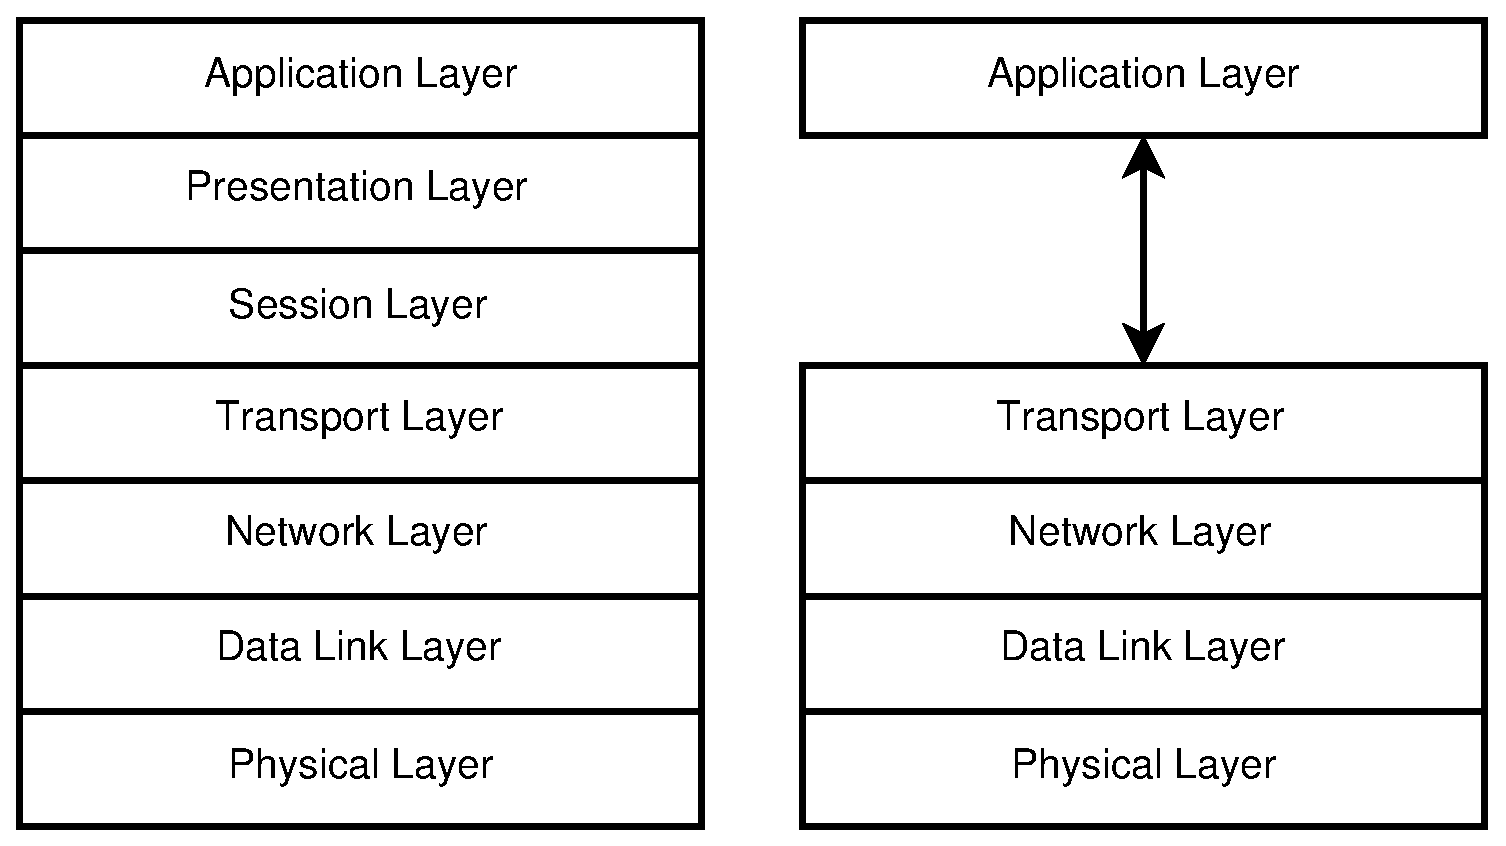
\includegraphics[width=0.7\textwidth]{figures/KNXvsISO.eps}
     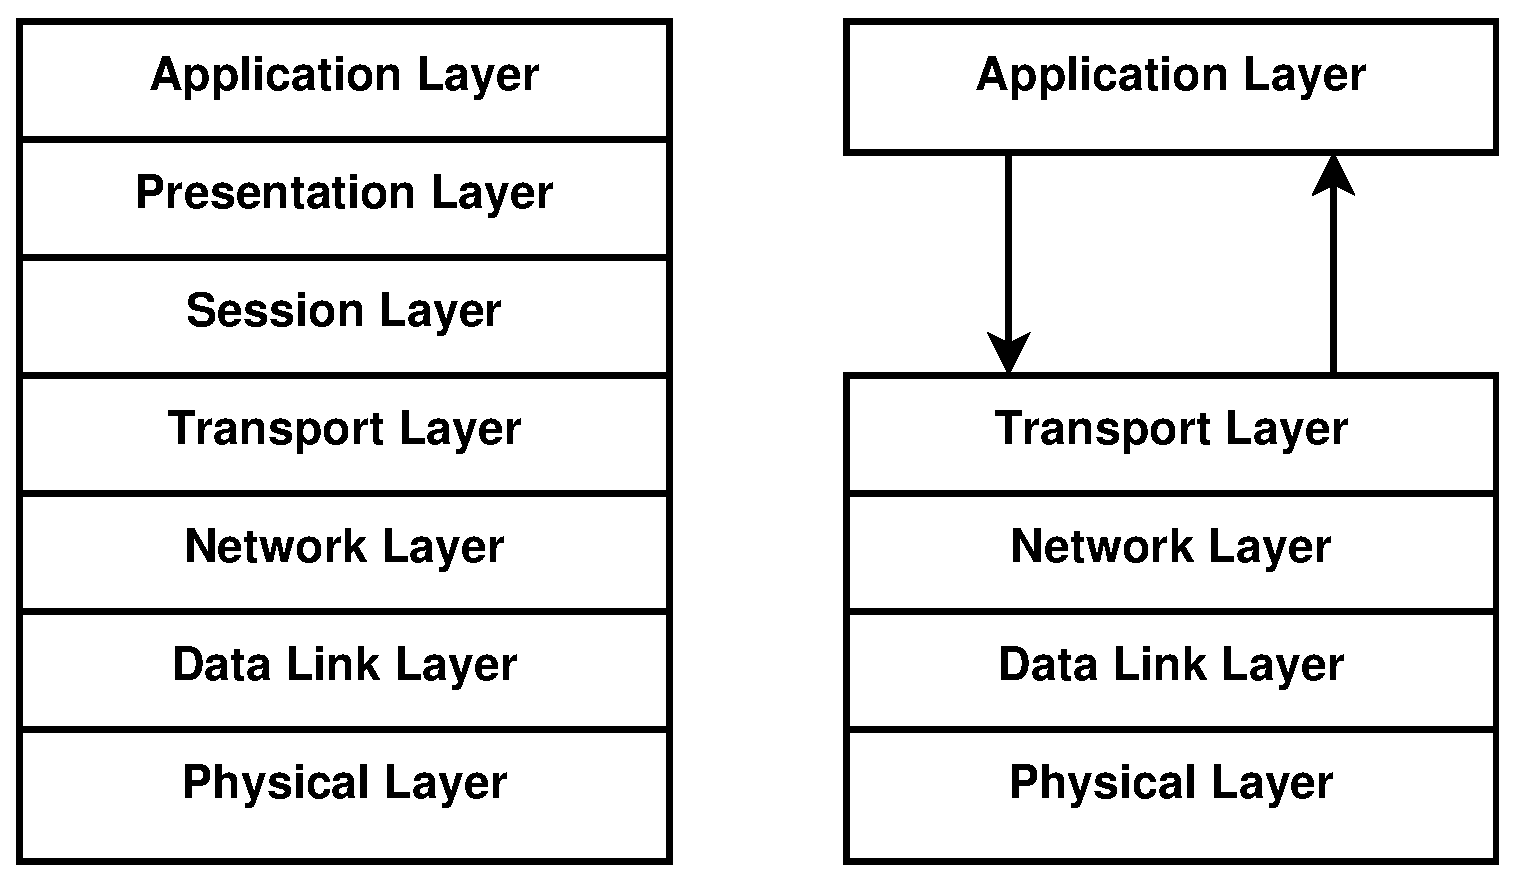
\includegraphics[width=0.7\textwidth]{figures/isoOSI.eps}

    \caption{OSI Layer Model, compared to the \gls{knx} Model}
    \label{fig:knxlayers}
\end{figure}

\subsection{Physical layer}
This is the lowest layer as defined by \gls{osi} and determines the basic transmission parameters like symbol rate, signal form but also mechanical 
characteristics like which connectors are used.
\\
\\
To provide flexibility in \gls{knx}, four different physical media are defined. \gls{TP}-1 which was inherited from \gls{eib}, and is the successor of \gls{TP}-0,
as defined by BatiBUS, is the basis medium, consisting of a twisted pair cabling. Data and power can be transmitted with one pair, so low-power
devices can be fed over the bus. Data transfer is done asynchronously, with bidirectional, half-duplex
communication and a datarate of 9600 \gls{bps}. \gls{TP}-1 uses collision avoidance, and allows all topologies beside rings. 
\\
Because this work is base on the \gls{TP}1 - part of \gls{knx} only, this medium will be explained in more detail in the next section.
\\
\\
PL110, which was also inherited from \gls{eib}, uses power line installations for communications. The carrier uses spread frequency shift keying, and can be used 
for bidirectional, half duplex  communication with an even lower data rate of 1200 bit/sec. \gls{knx} \gls{rf} is used for short range wireless communication
at 868,3 MHz. \gls{knx}net/\gls{ip} allows the integration of \gls{knx} into networks using \gls{TCP} / \gls{ip} for communication. Here, three different communication
modes are defined: tunneling mode is used for configuration and monitoring a client device by a \gls{knx}net/\gls{ip} server. Routing mode is used
for connecting \gls{knx} lines over \gls{ip}, while \gls{knx} \gls{ip} is used for direct communication between \gls{knx} devices. \cite{KraInnosec2013}

\subsubsection{TP-1}

The accurate name for this medium is 'Physical Layer type Twisted Pair', with variants
PhL \gls{TP}-1-64 and PhL \gls{TP}-1-256, which is backward compatible to the former one. While the first one allows
the connection of up to 64 devices, the latter one allows up to 256 devices connected in a linear, star, tree or
mixed topology as one physical segment, also called a line.
\\
Bridges do not possess their own address and are used for galvanic separation of physical segments and for extension of TP-1-64 segments to allow up to 256 devices.
Therefore, they acknowledge layer 2 frames received on one side and forward them to their second interface. 
\\
Routers have their own address space and only forward packages received on one side if the destination address is located on the other side of the router.
As well as bridges, they can be used for galvanic separation and they acknowledge frames on layer 2.
A \gls{lc} is a router that integrates up to 16 lines into one logical object called area. A \gls{bbc} is a router that connects
up to 16 areas to one network, thus providing the maximum size of a network consisting of 65536 devices:
\begin{itemize}
 \item up to 256 devices per line
 \item up to 16 lines per area = 4096 devices in 16 lines
 \item up to 16 areas for whole network = 65536\footnote{it is to be noted that the actual number of usable devices is smaller because routers have
 their own address} devices in 16 areas
\end{itemize}
Gateways are used to connect \gls{knx} networks to non-\gls{knx} networks.
\\
\\
A logical '1' is regarded as the idle state of the bus, so the transmitter of the \gls{mau} is disabled when sending a '1', i.e., the analog signal on
the bus consists only of the DC part. \gls{TP}-1 uses \gls{csma}/\gls{ca} for bus access, so every device must listen to the bus and is only allowed
to begin sending when the bus is idle. In the case of a simultaneous transmission start, a logical '1' of one
device will eventually be overwritten by a logical '0' of the other device. The overruled
sender will detect this by continuously checking the state of the bus and has to stop 
transmission. This behavior is be used to implement priority control and is exploited by the next layer.

\subsection{Data link layer for TP1}

This layer is responsible for error detection, retransmission of corrupted 
packages, framing of the higher level packages into suitable frames and accessing the bus according to the rules used by the particular bus medium. 
It is often broken into 2 distinct sublayers, namely the \gls{mac} as bus arbiter and the \gls{llc}, providing a reliable point-to-point datagram service.
\begin{figure}
    \centering
    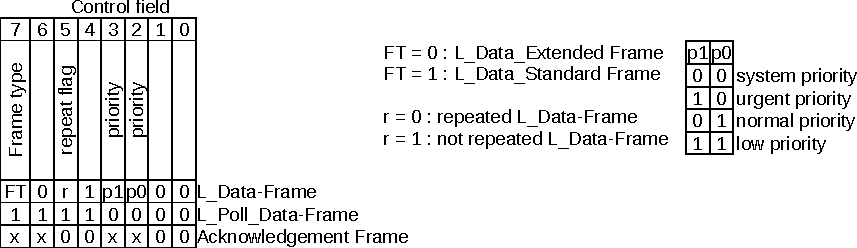
\includegraphics[width=1\textwidth]{figures/ctrl}
%    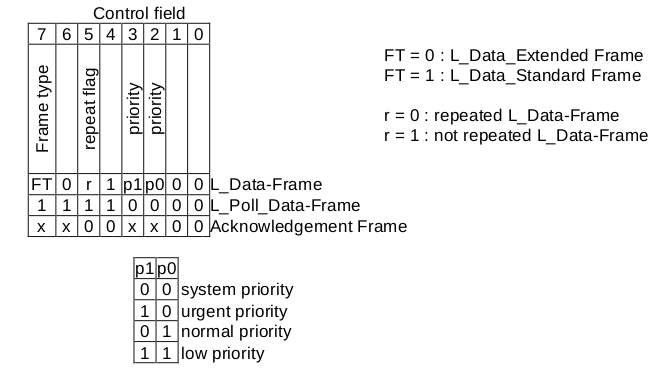
\includegraphics[width=0.5\textwidth]{figures/controlfield.png}
    \caption{Control Field}
    \label{fig:ctrlfield}
\end{figure}
Three frame formats are defined: L\_Data frames are used for sending a data payload to an \gls{ia}, a group address or for broadcasting data to
the bus. L\_Poll\_Data frames are used to request data from an individual \gls{knx} device or a group of devices. Acknowledgement frames are used to provide a reliable
transport mechanism, i.e., to acknowledge the reception of a frame by a \gls{knx} device. 
\\
For L\_Data\_Frame, 2 different formats are defined: standard frames, as shown in Figure \ref{fig:stdframe} and extended frames, see Figure \ref{fig:extframe}.
While standard frames can bear up to
15 bytes of application data, extended frames allow the transmission of up to 254 bytes of data.

\subsubsection{Standard L\_Data\_Frame}

Every standard frame starts with the control field, determining the frame type. 
After that, sender address and destination address, each 2 byte, follow.
The next byte contains 1 address type bit, 3 bits which belong to the \gls{lsdu} of the next higher layer
and 4 bits of length information, resulting in an maximum payload of 15 bytes(by design, it is also allowed to set this length
field to 0, i.e., to send an empty data frame). After the corresponding number of payload bytes, a check byte completes the frame. This check
frame is defined as an odd parity over all preceding bytes, which represents a logical NOT XOR function. 

\begin{figure}
    \centering
    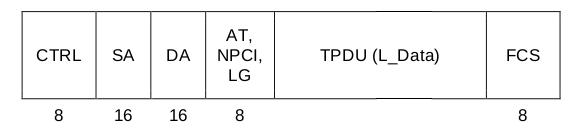
\includegraphics[width=0.8\textwidth]{figures/standardframe}
    \caption{Standard Frame}
    \label{fig:stdframe}
\end{figure}

\begin{figure}
    \centering
    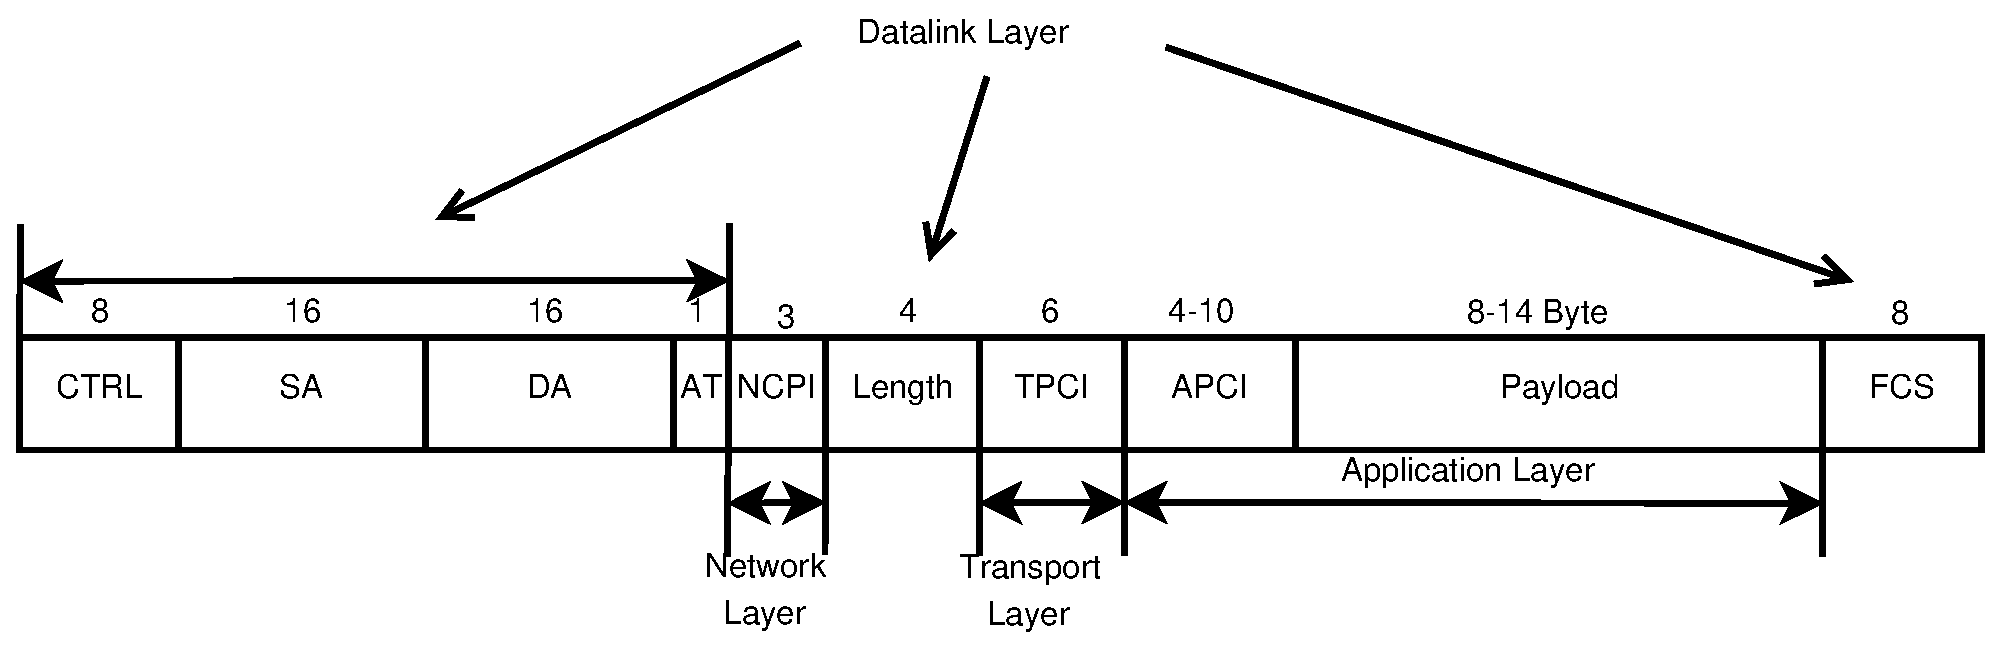
\includegraphics[width=0.8\textwidth]{figures/standardFrame.eps}
    \caption{Standard Frame, in detail}
    \label{fig:stdFrameDetail}
\end{figure}


\subsubsection{Extended L\_Data\_Frame}

The extended frame starts with a control field, as a standard frame. After that, a special \gls{ctrle} follows, as shown in Figure \ref{fig:ctrle}.
Source- and destination addresses, each 2 bytes, follow. To allow the bigger payload, the next byte is used as length field, with the value 0xFF reserved
as escape code, resulting in a maximum payload of 254 byte. After the length field, the payload and the check byte, as defined above, follow.

\begin{figure}
    \centering
    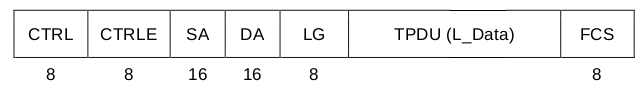
\includegraphics[width=0.8\textwidth]{figures/extendedframe}
    \caption{Extended Frame}
    \label{fig:extframe}
\end{figure}

\begin{figure}
    \centering
    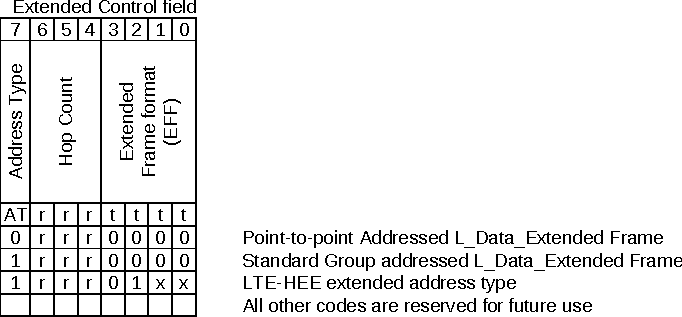
\includegraphics[width=0.8\textwidth]{figures/CTRLE}
    \caption{Extended Frame CTRLE field}
    \label{fig:ctrle}
\end{figure}

\subsubsection{L\_Poll\_Data frame}\label{sec:pollDataFrame}

These frames serve as data requests of the poll-data master for a maximum of 15 bytes
and start with a control field, as defined, followed by the 2 byte source address
of the sender (called Poll\_Data Master). The following 2 byte destination address is 
used to address up to 15 poll slaves, all belonging to the same poll group. The number of
exptected bytes and the check octet follow.
\\
Poll requests are answered by poll slaves by transmitting the databytes in the corresponding poll slave slot.
This is achieved by defining exact timings when each poll data slave must send the requested data. Therefore, such frames can only be used within
one physical segment \cite{knxTP1}.

\subsubsection{Acknowledge frame}\label{sec:ackFrame}

This frames are used to acknowledge the reception of a \gls{knx} data frames for \glspl{ga} or \glspl{ia} and consist
of one byte, sent after a fixed timespan after reception of the frame.

\subsection{KNX addressing scheme}

Two different kinds of addresses are defined: \glspl{ga} or \glspl{ia}, which type is used is determined by the 'address type' flag in the
control field of the datagram(0 = \gls{ia}). While the source address always is an \glspl{ia} and must be unique
within the network, the destination address can be of type group or individual (see Figure \ref{fig:knxAddr} for the layout).
\\
\\
For poll-data frames, the destination address determines the poll group address which must be unique within the physical segment.
\\
\\
Poll data responses as well as acknowledgement frames each just contain 1 byte, i.e., they do not possess source- and destination addresses.

\begin{figure}
 \centering
    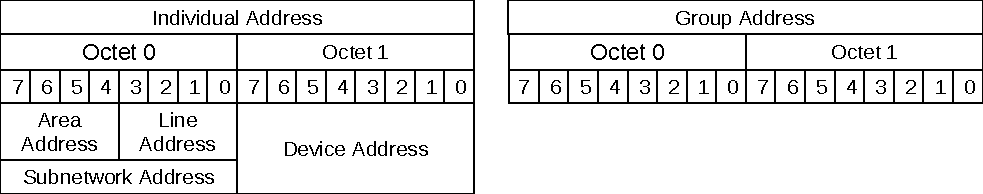
\includegraphics[width=0.9\textwidth]{figures/addresses}
 \caption{\gls{knx} individual and group addresses} 
\label{fig:knxAddr}
%% \subfloat[b]{0.3\textwidth}            
\end{figure}


\subsection{Network layer}

The main task of the network layer is the routing and forwarding of packets, so the main parameter on this layer is the destination address of the
datagram. Additionally, \gls{knx} reserves 3 bits of every standard- and extended data frame as
hop count. This counter is decremented by every router and the frame is discarded if the counter reaches the value zero. This mechanism, known from
\gls{ipv4} \cite{rfc791} \footnote{Originally, this was called \gls{ttl}}, avoids the infinite circulation of packages within an incorrectly configured network.

\subsection{Transport layer}\label{sec:knxTransportLayer}

Accoriding to the \gls{osi} modell, this layer provides point-to-point communication for hosts.
\\
In \gls{knx}, the connection orientated, reliable point-to-point communication mode addresses the \gls{ia} of a remote device and uses a timer to detect timeouts.
Up to to 3 retransmissions are allowed if the sent datagram is not acknowledged. A simple handshake - similar to \gls{tcp} - is used, as shown in Figure \ref{fig:handshake}.
\\
\\
All other modes are unreliable, i.e., unacknowledged, transport mechanisms and can be used to address a \gls{ia}, a \gls{ga} or all devices in the
network. For the latter mode, the special \gls{knx} broadcast address 0x0000 is reserved. 
The \gls{tpci}, included in the control field, determines the type of the \gls{tpdu} and also posseses a 4 bit sequence number by which duplicate datagrams, caused by damaged 
acknowledge-frames, can be discarded.

 \begin{figure}
    \centering
    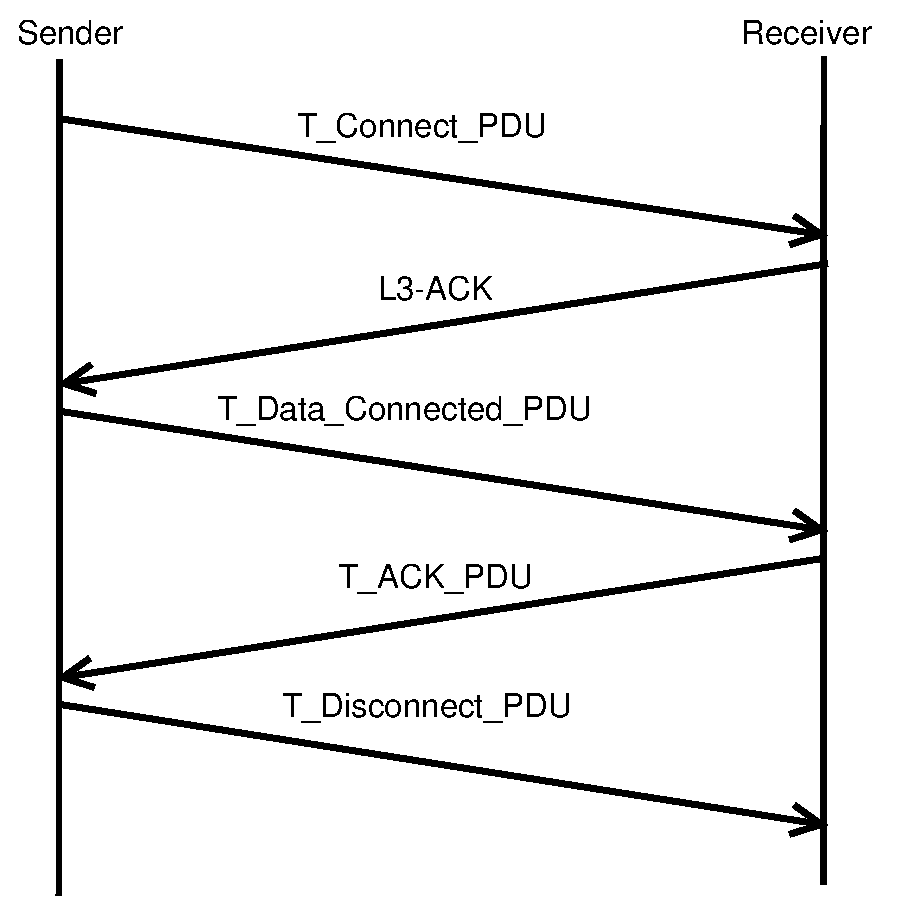
\includegraphics[width=0.5\textwidth]{figures/TransportHandshake.eps}
    \caption{Handshake for connection-orientated communication}
    \label{fig:handshake}
\end{figure}
 
\begin{figure}
    \centering
    \includegraphics[width=0.8\textwidth]{figures/"transport flags".png}
    \caption{Flags used at the Transport Layer}
    \label{fig:tFlags}
\end{figure}
%FIXME: quellenangabe bild, KNX standard

\subsection{Session layer}

This layer is responsible for maintaining sessions, i.e., it provides services to maintain synchronized data exchange. It does not exist in \gls{knx}.

\subsection{Presentation layer}

This layer allows a system-independent data representation, which is not necessary in \gls{knx} because the usage of standardized \glspl{dt}.

\subsection{Application layer}

This layer provides services for process-to-process information through a \gls{knx} network. Up to 10 bits are reserved in the application control field,
inside the \gls{apdu}, containing the application layer service code. The provided services range from tasks like reading or writing group values, distribution of network
parameters to obtaining device information.
